\documentclass[11pt]{article}

\usepackage[left=0.75in, right=0.75in, top=0.75in, bottom=0.75in]{geometry}
\usepackage{layout}
\usepackage{ucs}
\usepackage[utf8x]{inputenc}
\usepackage{titlesec}
\usepackage{graphicx}
\usepackage{amssymb}
\usepackage{amsmath}
\usepackage{dsfont}
\usepackage{float}
\usepackage{caption}
\usepackage{subcaption}
\usepackage{array}



\title{\textbf{TS113 - TP de communications numériques}}
\author{Maxime PETERLIN - Gabriel VERMEULEN\\\\{ENSEIRB-MATMECA, Bordeaux}}
\date{12 juin 2014}


\begin{document}

\maketitle
\tableofcontents

\newpage

\section{Communication numériques en bande de base}
	
	\subsection{Premier filtre de mise en forme}
		Dans cette partie, nous utiliserons le filtre de mise en forme suivant :
		\begin{equation}
			g(t) = 
			\left\{
		    	\begin{aligned}
		    		1&\,\,\,\,\,\, 0 \le t \textless T_s\\
		    		0&\,\,\,\,\,\, ailleurs
		      	\end{aligned}
		    \right.
		\end{equation}
		
		\subsubsection{Allure temporelle du signal $s_l(t)$}
			\begin{figure}[h]
				\centering
				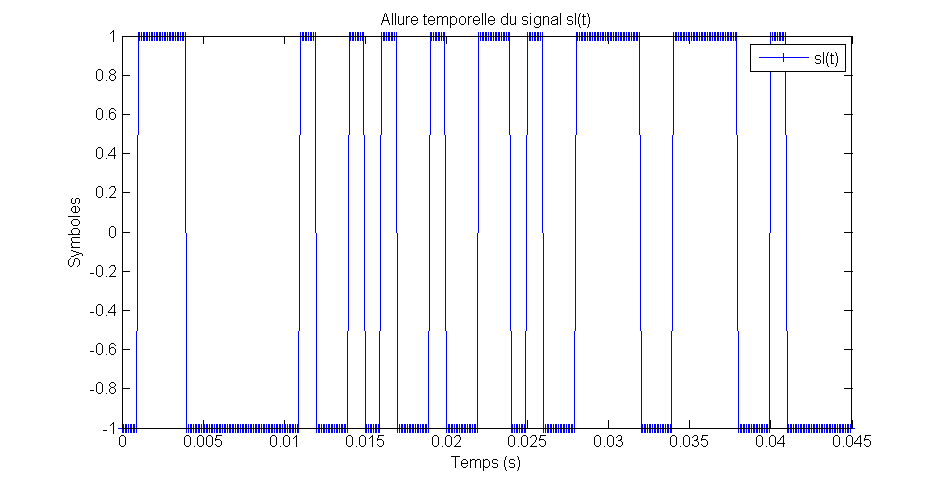
\includegraphics[scale=0.5]{images/Q311.png}
				\caption{Signal $s_l(t)$ pour $t \in [0, 50T_s-T_e]$}
				\label{Q311}
			\end{figure}
			$s_l$ est le signal en sortie du bloc correspondant à l'émetteur. \\
			La représentation temporelle de ce signal est directement liée au filtre de mise en fome où l'on retrouve le motif caractéristique de ce dernier.\\
			Cela se justifie notamment par la formule donnant $s_l$ : $s_l(t) = \sum\limits_{k \in \mathbb{Z}} A_kg(t-kT_s)$
			
		\subsubsection{Diagramme de l'oeil de $s_l(t)$}
			\begin{figure}[h]
				\centering
				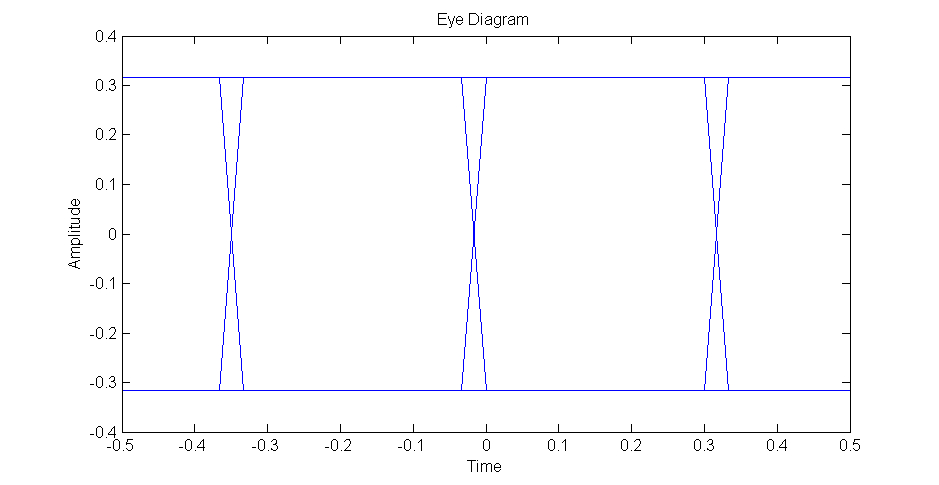
\includegraphics[scale=0.5]{images/Q312.png}
				\caption{Diagramme de l'oeil de $s_l(t)$ pour $3T_s$}
				\label{Q312}
			\end{figure}
			L'étude de la chaîne de communication se faisant sans bruit, il est normal de retrouver une ouverture de l'oeil qui soit maximale.\\
			De même l'ouverture horizontale est maximale, car l'échantillonneur n'induit pas de déphasage.
			
		\subsubsection{Allure temporelle du signal $r_l(t)$}
			\begin{figure}[h]
				\centering
				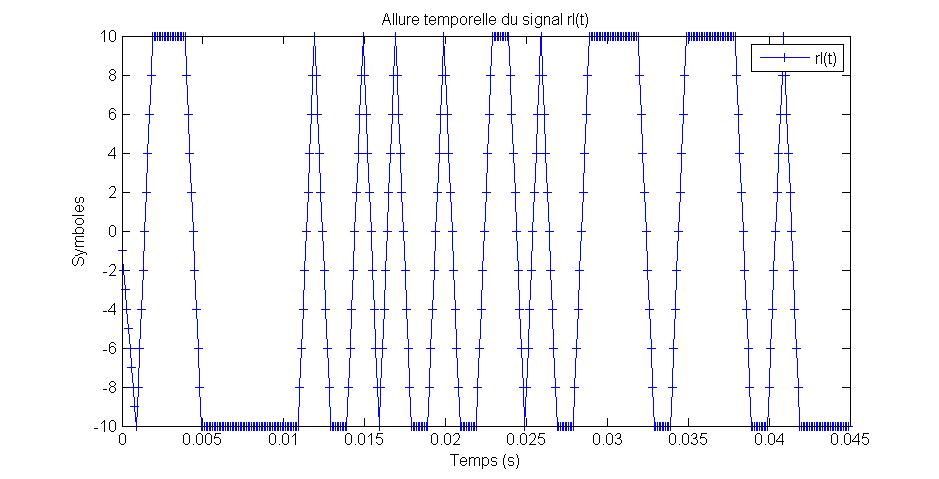
\includegraphics[scale=0.5]{images/Q313.png}
				\caption{Signal $r_l(t)$ pour $t \in [0, 50T_s-T_e]$}
				\label{Q313}
			\end{figure}
			Le signal réceptionné est échantillonné à une fréquence $F_{se}$.
		
		\subsubsection{DSP de $s_l(t)$ et $s_s(t)$}
			\begin{figure}[h]
				\centering
				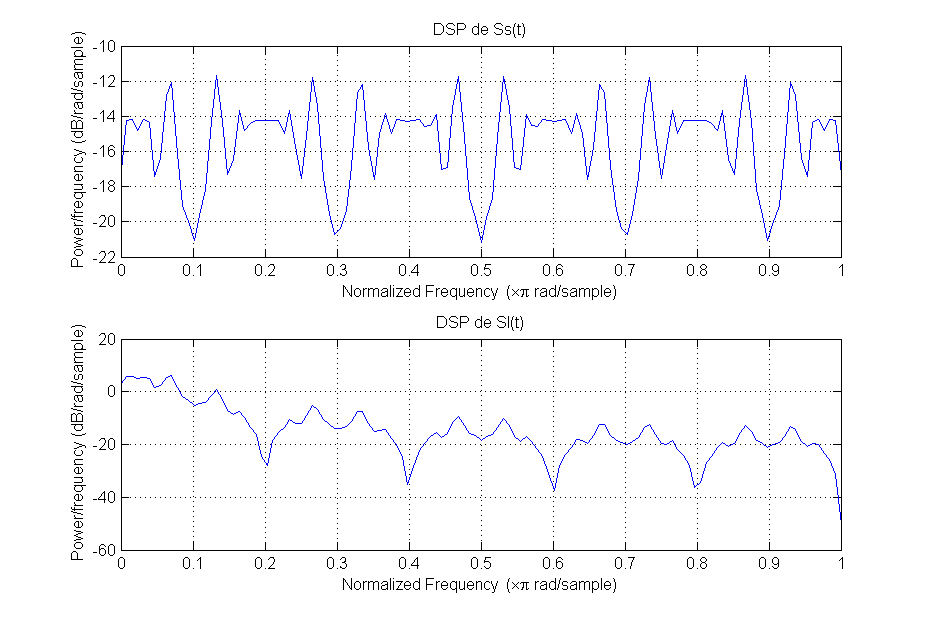
\includegraphics[scale=0.5]{images/Q314.png}
				\caption{Signal $r_l(t)$ pour $t \in [0, 50T_s-T_e]$}
				\label{Q314}
			\end{figure}
			
		
		\subsubsection{Évolution du TEB en fonction du rapport $\frac{E_b}{N_0}$}
			\begin{figure}[!ht]
				\centering
				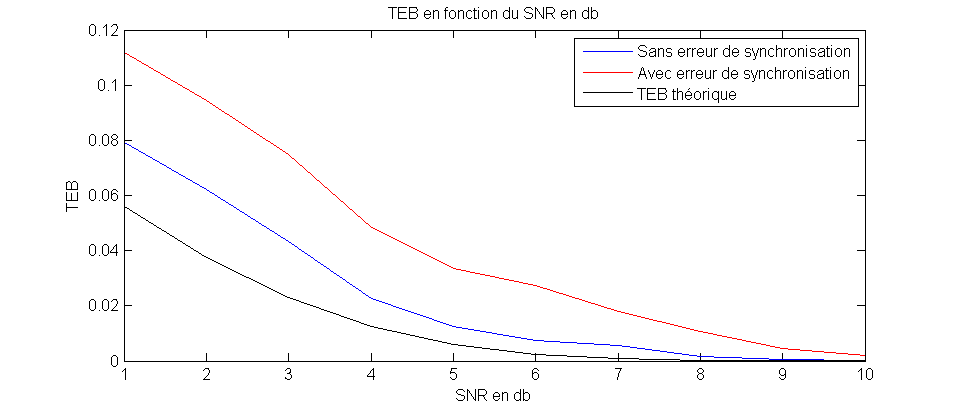
\includegraphics[scale=0.5]{images/Q315-6.png}
				\caption{Signal $r_l(t)$ pour $t \in [0, 50T_s-T_e]$}
				\label{Q315-6}
			\end{figure}
			On observe que le signal comportant une erreur de synchronisation en sortie du filtre adapté est naturellement placé au dessus de la courbe n'en possédant pas.\\
			De plus, à mesure que le SNR augmente, il est possible de quantifier cette erreur, car les erreurs binaires du signal sans erreur de synchronisation tendent vers 0.
			
			
		\subsubsection{Calcul de la perte de sensibilité du récepteur si le TEB $< 10^{-3}$}
	
	\subsection{Premier filtre de mise en forme}
		Dans cette partie, nous utiliserons le filtre de mise en forme suivant :
		\begin{equation}
			g_t(t) = 
			\left\{
		    	\begin{aligned}
		    		&(1-\frac{t}{T_s}) & \,\,\,\,\,\, 0 \le t \textless T_s\\
		    		&0 & \,\,\,\,\,\, ailleurs
		      	\end{aligned}
		    \right.
		\end{equation}
		
		\subsubsection{Allure temporelle du signal $s_l(t)$}
		\subsubsection{Diagramme de l'oeil de $s_l(t)$}
		\subsubsection{Allure temporelle du signal $r_l(t)$}
		\subsubsection{DSP de $s_l(t)$ et $s_s(t)$}
		\subsubsection{Évolution du TEB en fonction du rapport $\frac{E_b}{N_0}$}
		\subsubsection{Même manipulation avec une erreur de synchronisation temporelle}
		\subsubsection{Calcul de la perte de sensibilité du récepteur si le TEB $< 10^{-3}$}
		

\section{Communication numériques sur fréquence porteuse}
	\subsection{Étude théorique}
		\subsubsection{Modulateur et démodulateur numérique QPSK}
			Dans une transmission en QPSK, les symboles envoyés seront des nombres complexes et la phase de ces derniers sera l'information importante.\\\\
			La modulation passe par la génération d'une porteuse de fréquence $f_0$ que l'on va multiplier par ces symboles. Cette porteuse est, en général, une exponentielle complexe lors de simulation, mais en réalité il y a une différentiation entre ses parties réelles et complexes et est donc représentée respectivement par un cosinus et un sinus.\\
			Dans le cas de la simulation, on prend la partie réelle de la multiplication entre la porteuse et les symboles. On obtient alors un signal où, toutes les $T_s$ secondes, on a la porteuse avec une déphasage égal à l'argument du symbole correspondant à cet intervalle de temps.\\\\
			Le but de la démodulation va être d'identifier les déphasages des signaux compris entre les intervalles $kT_s$ et $(k+1)T_s$ du signal réceptionné.\\
			Pour cela on projette ce dernier sur un cosinus et un sinus de même fréquence pour obtenir respectivement le signal en phase et en quadrature de phase.\\
			On obtient alors les phases correspondantes aux différents symboles et, a fortiori, les symboles en eux-mêmes.
			
		\subsubsection{Expression théorique de la fonction de transfert $G(f)$ d'un filtre en racine de cosinus sur-élevé de roll-off $\alpha$}
			L'expression est la suivante :
				\begin{equation}
					G(f) = 
					\left\{
							\begin{aligned}
								&\frac{T_s}{2}(1-sin(\frac{\pi}{2\alpha}(2\lvert f \rvert T_s - 1)))&\,\,\,\,\,\, \frac{1-\alpha}{2T_s} \le \lvert f \rvert \le \frac{1+\alpha}{2T_s}\\
								&T_s&\,\,\,\,\,\, 0 \le \lvert f \rvert \le \frac{1-\alpha}{2T_s} \\
								&0&\,\,\,\,\,\, ailleurs
								\end{aligned}
						\right.
				\end{equation}
			
		
		\subsubsection{Expression de la DSP théorique de $s(t)$ lorsque le filtre de mise en forme est un filtre en racine de cosinus sur-élevé}
			$\Gamma_s(f) = \frac{1}{2T_s}\lvert G(f) \rvert^2$
		
	\subsection{Étude expérimentale - Canal à bande passante infinie}
		\subsubsection{Réponse impulsionnelle et module de la fonction de transfert du filtre en racine de cosinus sur-élevé}
			\begin{figure}[!h]
				\centering
				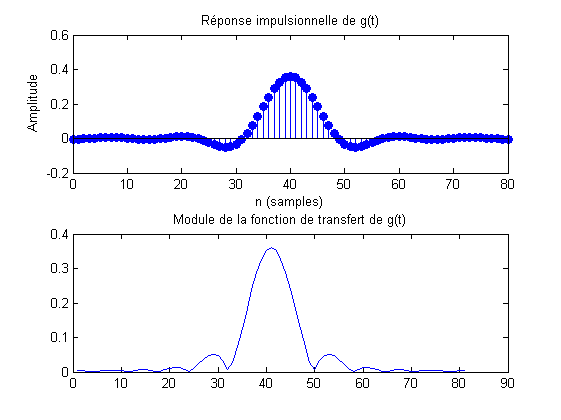
\includegraphics[scale=0.5]{images/Q421.png}
				\caption{Réponse impulsionnelle et module de la fonction de transfert}
				\label{Q421}
			\end{figure}
			
		
		\newpage
		\subsubsection{Diagramme de l'oeil de $s_l(t)$}
			\begin{figure}[!h]
				\centering
				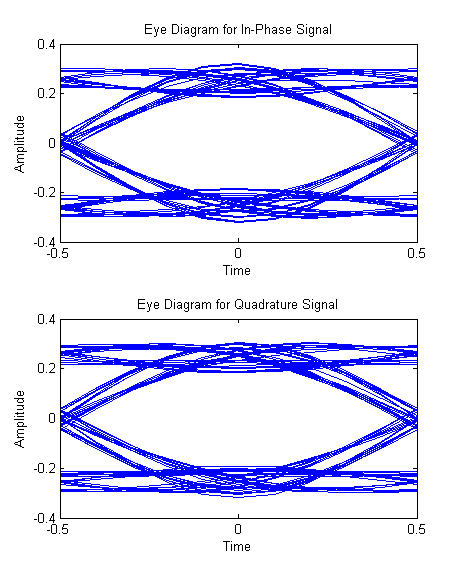
\includegraphics[scale=0.5]{images/Q424.png}
				\caption{Diagramme de l'oeil de $s_l(t)$}
				\label{Q424}
			\end{figure}
		On représente ici les diagrammes de l'oeil des signaux en phase et en quadrature composants le signal $s_l(t)$.\\
			On remarque que l'ouverture verticale de l'oeil n'est pas maximal de même que pour l'ouverture horizontale, alors que la simulation se fait sans bruit. Cependant, il y a effectivement des déphasages, car c'est le propre de la modulation QPSK.
			
		\subsubsection{Diagramme de l'oeil de $r_l(t)$}
			\begin{figure}[!ht]
				\centering
				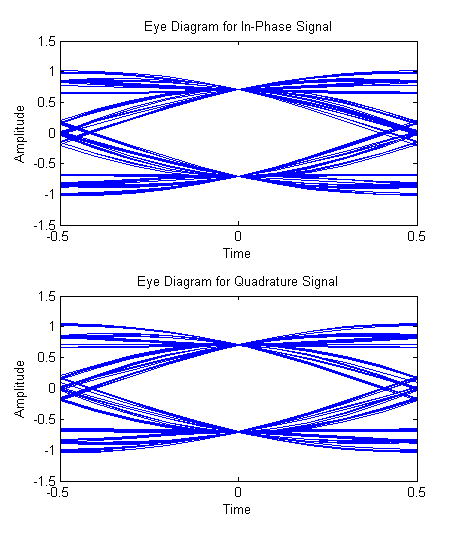
\includegraphics[scale=0.5]{images/Q425.png}
				\caption{Diagramme de l'oeil de $r_l(t)$}
				\label{Q425}
			\end{figure}
		On représente ici les diagrammes de l'oeil des signaux en phase et en quadrature composants le signal réceptionné $r_l(t)$.\\
			On remarque que l'ouverture verticale de l'oeil est ici maximale comparée au diagramme de l'oeil de $s_l(t)$. On remarque également que l'ouverture horizontale n'est pas maximale, car le signal comporte des déphasages.
			
		\subsubsection{Constellations de $s_s(t)$ et $r_l[n]$}
			\begin{figure}[!h]
				\centering
				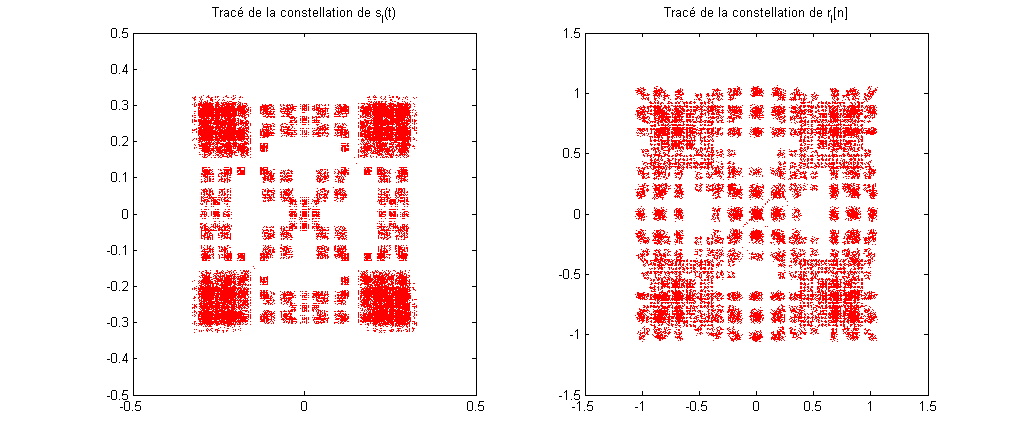
\includegraphics[scale=0.5]{images/Q426.png}
				\caption{Constellations de $s_s(t)$ et $r_l[n]$}
				\label{Q426}
			\end{figure}
			Dans les deux constellations, on repère bien les positions des différents symboles complexes. Cependant, ces dernières sont parsemées de points résiduels.\\
			Dans le cas du signal $s_l$, ces points proviennent du filtre de mise en forme et pour $r_l[n]$ cela provient de l'échantillonnage. 
			
		\subsubsection{Partie réelle de $r_l(t)$}
		
		
		\subsubsection{Comparaison entre la DSP théorique de $s(t)$ avec la DSP expérimentale}
		
		\subsubsection{DSP de $y_l(t)$}
			\begin{figure}[!h]
				\centering
				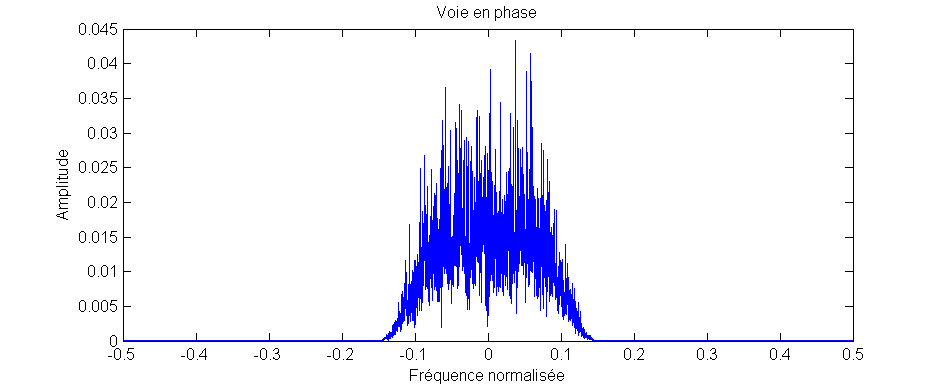
\includegraphics[scale=0.5]{images/Q4211.png}
				\caption{DSP de $y_l(t)$}
				\label{Q4211}
			\end{figure}
			
			

\end{document}
